\section{Introdução}

O TerraMax é um veículo militar autônomo precursor de diversas tecnologias de autonomia voltada para veículos militares terrestres existentes hoje em dia. Desenvolvido pela equipe Oshkosh, o veículo participou dos desafios da DARPA (\emph{Defense Advanced Research Projects Agency}) em 2004, 2005 e 2007.

Este documento relata o desenvolvimento do veículo autônomo, com foco no desafio de 2007, o DARPA Urban Challenge, no qual o robô deve trafegar em vias urbanas respeitando leis de trânsito e cumprindo diversas manobras desafiadoras sem interferência humana. As principais informações relativas ao veículo relatadas aqui foram retiradas das referências \cite{chen2009terramax}, \cite{braid2006terramax} e \cite{broggi2008passive}.

Nesta seção introdutória, serão apresentados um breve histórico do robô, as motivações e objetivos por trás de seu desenvolvimento, a equipe desenvolvedora, e uma visão geral do veículo e o \emph{hardware} utilizado.

\subsection{Motivações e Objetivos}

O TerraMax é o único veículo, dentre todos os participantes dos DARPA \emph{Grand Challenge} (DGC) de 2004, 2005 e 2007, voltado para a aplicação militar. O objetivo da equipe Oshkosh era desenvolver tecnologia de robótica autônoma para aplicação em veículos militares terrestres com a motivação de aprimorar o suporte logístico de cargas pesadas em campos de batalha.

Tendo isso em mente, a equipe desenvolveu o robô de modo a não somente satisfazer critérios de performance nos desafios como também torná-lo apto à operação em campo. Desse modo, a escolha do \emph{hardware} e o desenvolvimento dos algoritmos de navegação considerou a aplicação militar na prática. Por exemplo, os computadores embarcados selecionados são robustos, para condições ``ultra-harsh", com encapsulamentos com certificações IP, resistência a impacto e vibração, entre outros.

Outro objetivo da equipe era desenvolver um sistema modular, de forma que novas funcionalidades poderiam ser incluídas no veículo com facilidade, e que o mesmo sistema pudesse ser utilizado para diferentes veículos militares.

\subsection{Histórico}

O TerraMax participou do desafio de 2004, em que nenhuma equipe conseguiu completar os objetivos da prova, e do DGC \emph{off-road} de 2005, antes de sua participação no DGC urbano de 2007.

A equipe realizou mudanças significativas de 2004 para 2005, como na direção das rodas traseiras para melhor desempenho em curvas acentuadas, e a completa reformulação do sistema autônomo. O TerraMax completou o desafio \emph{off-road} na quinta posição, após 28h ininterruptas de operação com sucesso em desvio de obstáculos e navegação em diferentes situações de estrada.

Para o desafio urbano, a equipe incluiu novos sensores (câmeras e LIDARs), sobretudo nas laterais e na traseira do veículo, de modo a adequar o sistema para navegação urbana. No ambiente \emph{off-road} do DCG 2005, não era necessário o sensoriamento lateral e traseiro, o que é de extrema importância no ambiente urbano para que o veículo lide com situações de ultrapassagem e cruzamentos, por exemplo.

\subsection{Equipe do DGC 2007}

Para o desafio urbano de 2007, a equipe foi incrementada com as participações da Teledyne e da Universidade de Auburn. As equipes e respectivas atribuições são descritas abaixo.

A \textbf{Oshkosh Corporation} é uma empresa americana voltada para a área de defesa, sendo a principal responsável pelo projeto. Suas atribuições no projeto foram providenciar o veículo, lidar com o gerenciamento do projeto, realizar a integração eletromecânica e o controle de \emph{software} de médio/baixo nível.

A \textbf{Teledyne Scientific and Imaging Company} é uma empresa americana de alta tecnologia voltada para pesquisa, desenvolvimento em sistemas de informação e sensoriamento de imagem para aplicações militares, espaciais e comerciais. No DGC 2007, foi responsável pelo \emph{software} de alto nível, ou seja, o comportamento autônomo do veículo, o que inclui controle de missão, planejamento de trajetórias e supervisão.

O laboratório \textbf{VisLab}, da Universidade de Parma, na Itália, continuou no projeto com a responsabilidade de desenvolver os sistemas de visão. Juntamente com os dados dos LIDARs, o sistema de visão compõe a principal parte de percepção do veículo.

A alemã \textbf{Ibeo Automotive Sensor} providenciou os LIDARs e a integração desses sensores com o \emph{software} desenvolvido para o veículo. Finalmente, a \textbf{Universidade de Auburn}, nos Estados Unidos, ficou responsável pelo desenvolvimento do sistema inercial e de GPS.

\subsection{Veículo e Visão Geral do \emph{Hardware}}

O TerraMax é uma versão adaptada de um veículo terrestre militar, um Medium Tactical Vehicle Replacement (MTVR), produzido pela Oshkosh. A equipe removeu boa parte da caçamba e o terceiro eixo de veículo, além de incluir suspensões no eixo traseiro para permitir melhor mobilidade em curvas estreitas no ambiente urbano. A \reffig{fig:veiculo} compara o veículo original com o adaptado.

\begin{figure}[h]
\centering
\subfloat{\myfboxthin{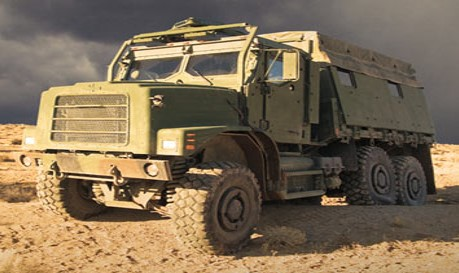
\includegraphics[height=0.375\columnwidth]{figs/MTVR.jpg}}}\enskip
\subfloat{\myfboxthin{\includegraphics[height=0.375\columnwidth]{figs/TerraMax.jpg}}}
\caption{Veículo MTVR original (esq.) e TerraMax (dir.).}%
\label{fig:veiculo}%
\end{figure}

A direção, aceleração e freio do veículo também foram adaptados para o sistema \emph{drive by wire}, e o sistema embarcado (computadores e eletrônica) foi instalado abaixo do assento do passageiro \reffigp{fig:EE}. Além disso, diversos sensores foram instalados ao redor do veículo, como será descrito mais adiante.

%Computadores
Foi utilizado um total de 6 computadores embarcados disponíveis comercialmente (\emph{commercial off-the-shelf}), além de controladores de baixo nível customizados pela Oshkosh. Dois computadores embarcados (A-Plus Mobile A20-MC) robustos e apropriados para ambientes rigorosos foram utilizados para o comportamento autônomo do veículo, rodando Windows XP como sistema operacional. Um computador SmallPC Core Duo, também com certificação IP, foi usado para cada um dos quatro sistemas de visão do veículo, rodando Linux Fedora. As Figuras \ref{fig:EE} e \ref{fig:computadores} mostram os modelos utilizados.

\begin{figure}[!h]
\centering
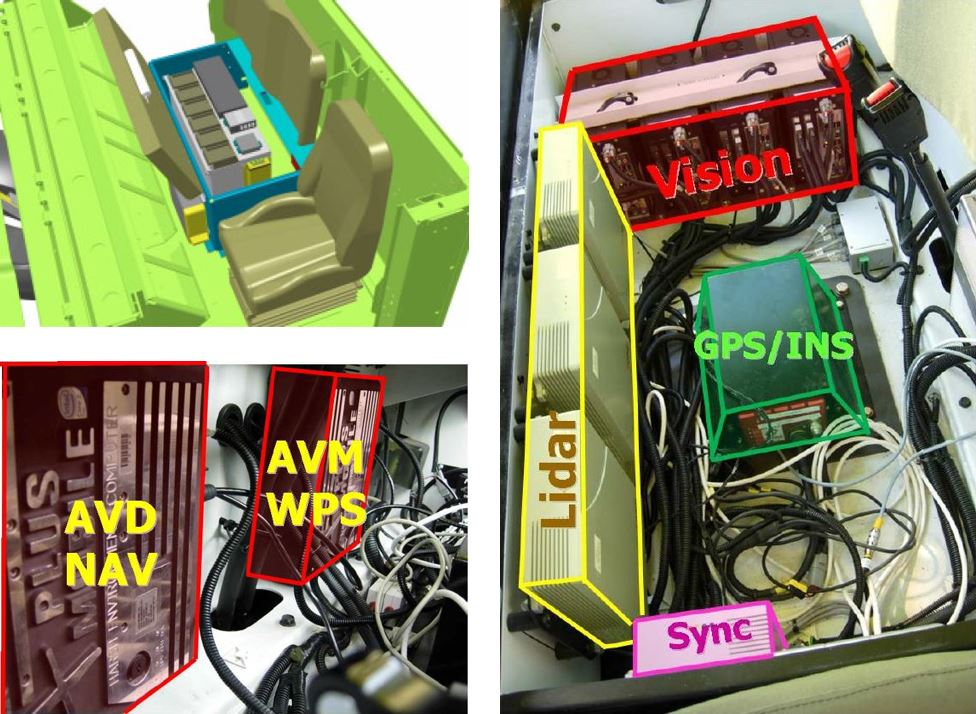
\includegraphics[width=0.75\columnwidth]{figs/EE.jpg}
\caption{Computadores embarcados robustos utilizados no TerraMax.}%
\label{fig:EE}%
\end{figure}

\begin{figure}[!h]
\centering
\subfloat{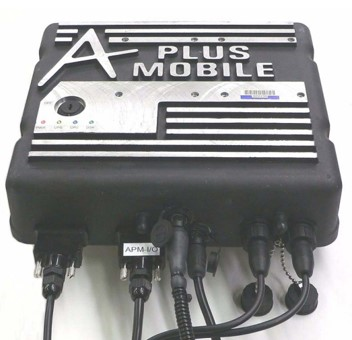
\includegraphics[height=0.375\columnwidth]{figs/Aplus.jpg}}\quad
\subfloat{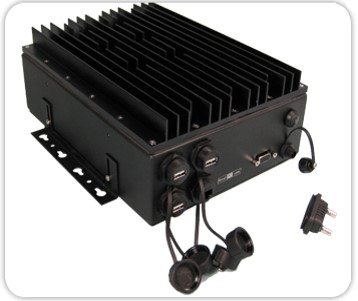
\includegraphics[height=0.375\columnwidth]{figs/SmallPC.jpg}}
\caption{Computadores embarcados robustos utilizados no TerraMax.}%
\label{fig:computadores}%
\end{figure}

O sistema de sensoriamento do TerraMax conta com 3 LIDARs (2 frontais e 1 traseiro), 11 câmeras instaladas ao redor do veículo e um sistema de navegação inercial com duas antenas GPS posicionadas na parte superior. A \reffig{fig:sensores} destaca o local de instalação desses sensores no veículo.

\begin{figure}[h]
\centering
\subfloat{\myfboxthin{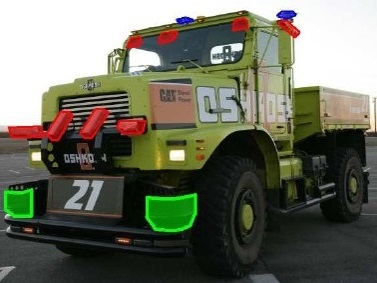
\includegraphics[height=0.3\columnwidth]{figs/front.jpg}}}\enskip
\subfloat{\myfboxthin{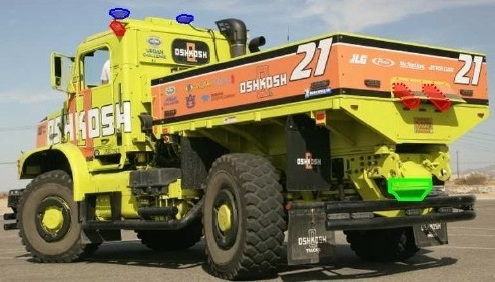
\includegraphics[height=0.3\columnwidth]{figs/rear.jpg}}}
\caption{Visão frontal e traseira do TerraMax, com destaque para os sensores instalados: câmeras (vermelho), LIDARs (verde) e antenas GPS (azul).}%
\label{fig:sensores}%
\end{figure}

Os objetivos e descrição de cada sistema de sensoriamento, bem como o hardware utilizado, serão detalhados na \refsec{sec:perception}.


